\documentclass[tikz]{standalone}
\usepackage{times}
\usepackage{amsmath}
\usepackage{txfonts}
\usepackage{xcolor}
\usepackage[utf8]{inputenc}
\usepackage{graphics}
\usepackage{pgfplots}
\usetikzlibrary{spy}
\usetikzlibrary{calc}
\usetikzlibrary{arrows.meta}
\usetikzlibrary{patterns}
\usetikzlibrary{pgfplots.fillbetween}
\usepackage{ifthen}
\begin{document}
	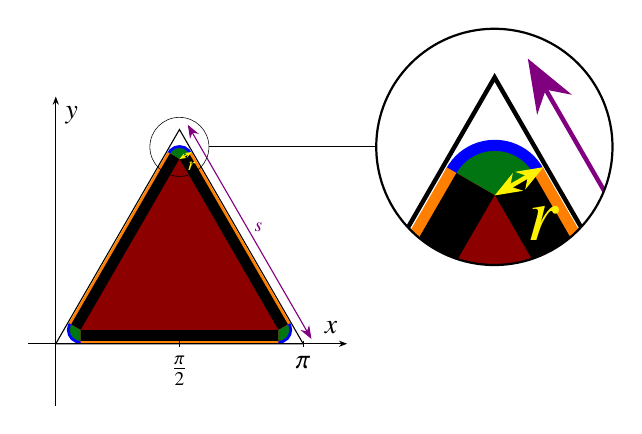
\begin{tikzpicture}[spy using outlines={circle, magnification=4, size=3cm, connect spies}]
		\definecolor{clrGreen}{RGB}{0, 117, 18}
		\definecolor{darkred}{rgb}{0.55, 0.0, 0.0}
		
		\def\sidelength{3.14159}
		
		\pgfmathsetmacro{\triangleheight}{sqrt(3)/2*\sidelength}
		
		\draw[fill=white] (0,0) -- (\sidelength,0) -- (0.5*\sidelength, \triangleheight) -- cycle;
		\coordinate (A) at (0,0);
		\coordinate (B) at (2.51,0);
		\coordinate (C) at (2.51/2,1.73/2*2.51);
		
		\coordinate (As) at ($(A) + (9pt,5pt)$);
		\coordinate (Bs) at ($(B) + (9pt,5pt)$);
		\coordinate (Cs) at ($(C) + (9pt,5pt)$);
		
		\node[circle, inner sep=0pt, minimum size=9pt, fill=clrGreen, draw=blue, line width=1pt] at (As) {};
		\node[circle, inner sep=0pt, minimum size=9pt, fill=clrGreen, draw=blue, line width=1pt] at (Bs) {};
		\node[circle, inner sep=0pt, minimum size=9pt, fill=clrGreen, draw=blue, line width=1pt] at (Cs) {};
		
		\draw[line width=10pt, orange] (As) -- (Bs) (Bs) -- (Cs) (Cs) -- (As);
		\draw[line width=8pt, black] (As) -- (Bs) (Bs) -- (Cs) (Cs) -- (As);
		
		\path[fill=darkred] (As) -- (Bs) -- (Cs) -- (As);
		
		\draw[<->,thin, yellow,>={Stealth[scale=0.5]}] (0.5*\sidelength, \triangleheight-0.375) -- (0.5*\sidelength+0.155, \triangleheight-0.285) node[below] {\scriptsize$r$};
		
		\draw[<->, thin, violet,>={Stealth[scale=1]}] ([shift={(+3pt,1.7pt)}]\sidelength,0) -- ([shift={(3pt,1.7pt)}]0.5*\sidelength, \triangleheight) node[] at ([shift={(6pt,3.4pt)}]0.75*\sidelength,0.5*\triangleheight) {\scriptsize$s$};
		
		\draw[->,thin,>={Stealth[scale=0.62]}] (-0.35,0) -- (3.7,0) node[above left] {$x$};
		\draw[->,thin,>={Stealth[scale=0.62]}] (0,-0.785) -- (0,3.14) node[below right] {$y$};
		
		\foreach \x/\xlabel in {1.5708/$\frac{\pi}{2}$, 3.14159/$\pi$}
		\draw (\x,1pt) -- (\x,-1pt) node[below] {\xlabel};
		
		\spy on (1.57,2.5) in node [right] at ($(1.57,2.5)+(2.5,0)$);
	\end{tikzpicture}
\end{document}